\documentclass[../../main.tex]{subfiles}

\begin{document}

\chapter{Results} \label{chapter:results}

A number of experiments were conducted with two broad goals: verifying that at least some of the proposed architecture works on simplified abstract engineering environments, and proving that it has desirable qualities in more complex environments.
Some experiments were also carried out to visualise and explore the latent space mappings in an intuitive way.

\section{Approach verification} \label{section:approachVerification}

\subsection{Distribution distance} \label{subsection:distributionDistance}

Due to the potential issues with minimising KL-divergence discussed in \S\ref{subsection:potentialIssues}, a simplified environment was devised in which the target distribution $\hat{V_c}$ is known.
$\hat{V_c}$ was fixed as a standard normal distribution (constraints were not considered at this stage) and $\hat{V'_c}$ was modelled as a normal distribution whose mean and standard deviation were learned parameters.

Although KL-divergence is analytically tractable for two normal distributions, it was estimated through sampling of $\hat{V'_c}$ as described in \S\ref{subsection:klDivergence}.
Initial standard deviation $\sigma_0$ was always set to $1$, while initial mean $\mu_0$ was varied.
\begin{figure}[H]
    \begin{center}
    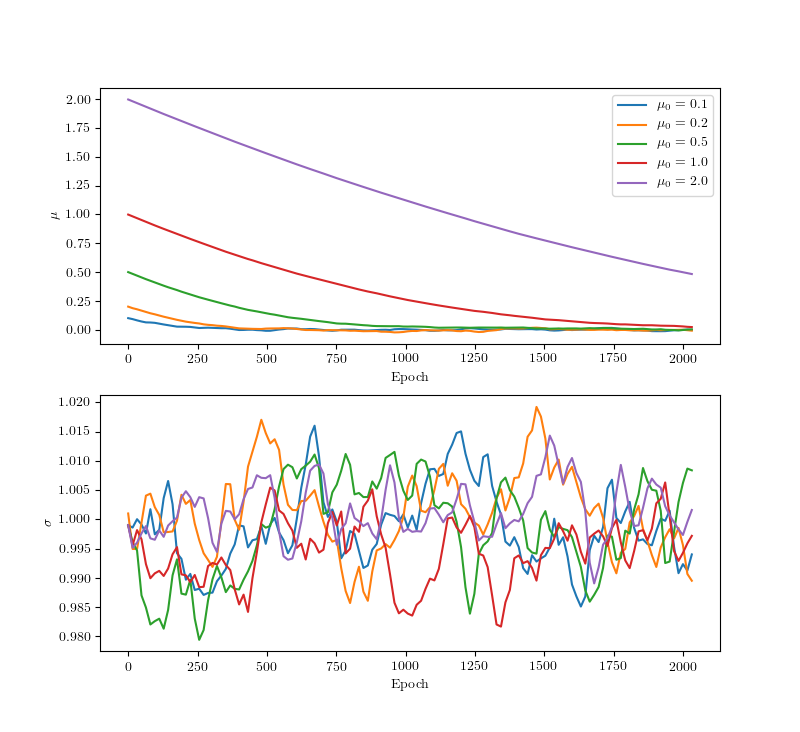
\includegraphics[width=\textwidth]{broadKLDivergence}
    \caption{
        Change in $\mu$ and $\sigma$ over time when training arbitrary normal distributions with different starting means to match the standard normal distribution.
        Training parameters are reproduced in Appendix \ref{appendix:klTrainingParameters}.
    }
    \label{fig:broadKLDivergence}
    \end{center}
\end{figure}
The mean $\mu$ and standard deviation $\sigma$ after each batch are shown in Figure \ref{fig:broadKLDivergence}.
Convergence does occur, but the time taken for the mean to approach $0$ appears to increase exponentially as the initial mean moves away from the target.
Two one-dimensional normal distributions whose means only differ by two and whose standard deviations are both one could still be considered to be quite similar, so the experiment was repeated with $\sigma_0=0.1$ for both distributions to better simulate disjoint distributions.
\begin{figure}[H]
    \begin{center}
    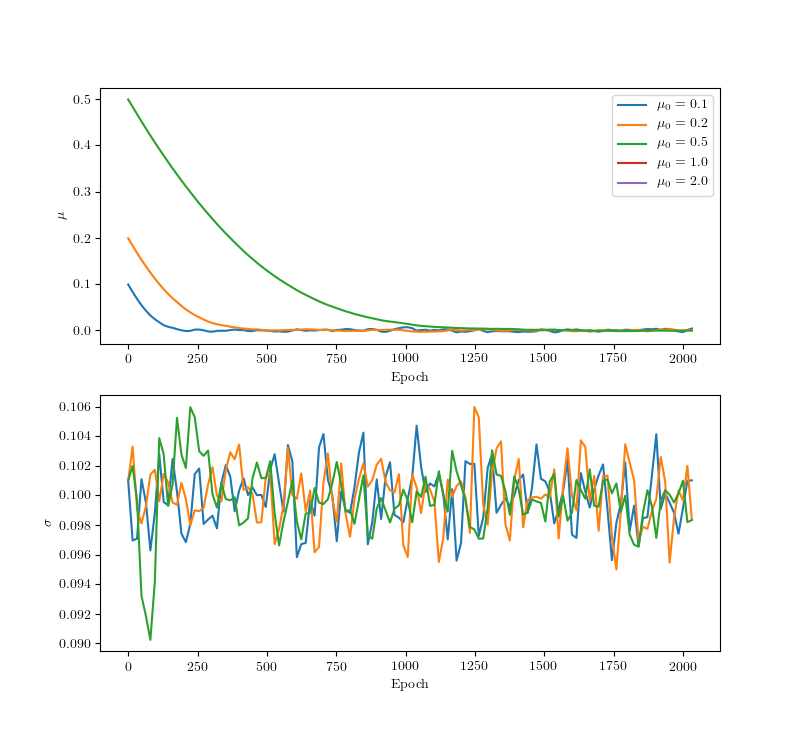
\includegraphics[width=\textwidth]{narrowKLDivergence}
    \caption{
        Change in $\mu$ and $\sigma$ over time when training arbitrary normal distributions with different starting means to match a normal distribution with $\mu=0$ and $\sigma=0.1$. 
        Training parameters are reproduced in Appendix \ref{appendix:klTrainingParameters}.
    }
    \label{fig:narrowKLDivergence}
    \end{center}
\end{figure}
Figure \ref{fig:narrowKLDivergence} shows that the variables converge at approximately the same rate as when $\sigma_0=1$.
Both $\mu$ and $\sigma$ went to \url{NaN} after the first epoch and so are not shown.
This may well have been caused by an excessively large KL-divergence resulting in exploding gradients due to the limited precision of floating point numbers.

Changing to 64- instead of 32-bit values lends further evidence to this hypothesis, as increasing the precision allowed the $\mu=1.0,2.0$, $\sigma=0.1$ cases to be optimised without numerical errors (Figure \ref{fig:narrowKLDivergenceFloat64}).
Similarly, using 16-bit precision always resulted in \url{NaN} errors occurring.
\begin{figure}[H]
    \begin{center}
    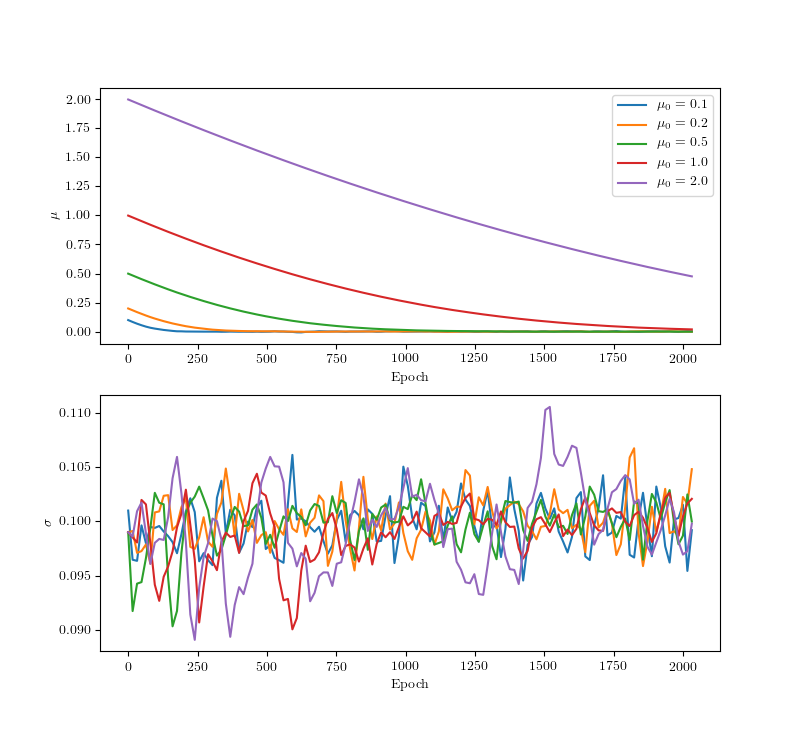
\includegraphics[width=\textwidth]{narrowKLDivergenceFloat64}
    \caption{
        Change in $\mu$ and $\sigma$ over time when training arbitrary normal distributions with different starting means to match a normal distribution with $\mu=0$ and $\sigma=0.1$. 
        Training parameters are those in Appendix \ref{appendix:klTrainingParameters}, but with 64-bit precision.
    }
    \label{fig:narrowKLDivergenceFloat64}
    \end{center}
\end{figure}
It was therefore concluded that minimising KL-divergence is too inconsistent for practical use, as real distributions $-$ which are frequently disjoint $-$ would very likely cause numerical issues due to lack of the required precision.

\subsection{Precision proxy optimisation} \label{subsection:precisionProxyOptimisation}

All experiments in this section used the parameters in Appendix \ref{appendix:precisionOptimisationTrainingParameters}.

Potential issues with directly estimating $\hat{r}$ were discussed in \S\ref{section:neuralNetworkInversion}.
It was also hypothesised that optimising only $\hat{p}$ would result in $g'$ sampling only a small subset of $V_c$.
A short experiment was devised to prove that this is the case and so a substitute for $\hat{r}$ would be needed.
$h$ was defined arbitrarily for $m=1,\;n=0$, described in detail in Appendix \ref{appendix:unimodalCSF}.
A graph of the constraint satisfaction function on $s\in[-1,\;1]$ is shown in Figure \ref{fig:sigmoidBumpFunction}.
\begin{figure}[H]
    \begin{center}
    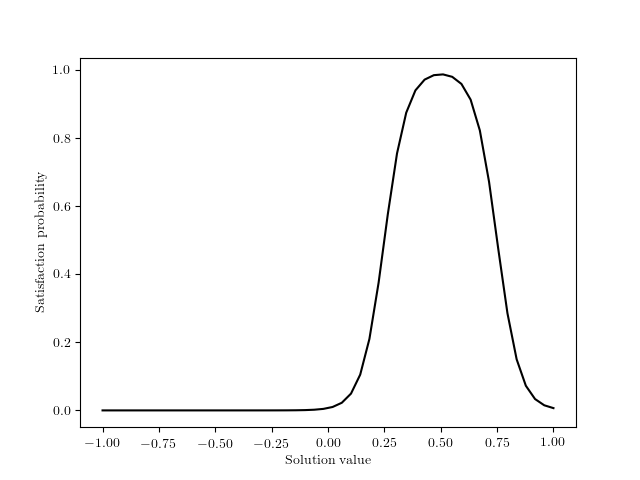
\includegraphics[width=\textwidth]{sigmoidBumpFunction}
    \caption{
        A test function estimating the probability that a solution satisfies a singular constraint.
    }
    \label{fig:sigmoidBumpFunction}
    \end{center}
\end{figure}
Optimising $g'$ against $h(c,s)$ for $\hat{p}$ consistently yields a distribution of generated solutions displayed in Figure \ref{fig:sigmoidBumpHistogram}.
Only considering precision and disregarding recall produces a mapping which is of no use: it always maps to a singular point in spite of the fact that around $15\%$ of the solution space has a constraint satisfaction probability above $0.9$.
\begin{figure}[H]
    \begin{center}
    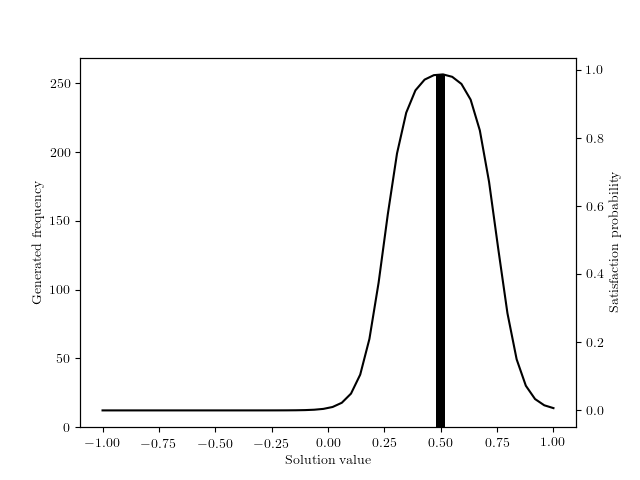
\includegraphics[width=\textwidth]{sigmoidBumpHistogram}
    \caption{
        Histogram of samples from $\hat{V'_c}$ compared to $h$ after optimising only $\hat{p}$.
    }
    \label{fig:sigmoidBumpHistogram}
    \end{center}
\end{figure}
This issue becomes more pronounced when $h$ has two distinct modes (Figure \ref{fig:sigmoidBumpHistogramBimodal}, Appendix \ref{appendix:bimodalCSF}).
While a very high precision is obtained, optimising solely for precision fails to capture the bimodality of $h$ even in a simple environment, confirming that optimisation must take recall into consideration for satisfactory results.
\begin{figure}[H]
    \begin{center}
    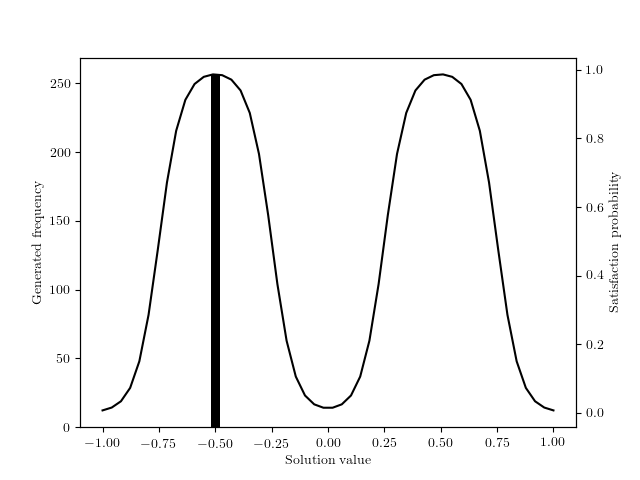
\includegraphics[width=\textwidth]{sigmoidBumpHistogramBimodal}
    \caption{
        Histogram of samples from $\hat{V'_c}$ compared to $h$ after optimising only $\hat{p}$.
    }
    \label{fig:sigmoidBumpHistogramBimodal}
    \end{center}
\end{figure}

\subsection{Pretraining} \label{subsection:pretrainingResults}

All experiments in this section used the parameters in Appendix \ref{appendix:precisionOptimisationTrainingParameters} unless otherwise specified.

Without $\hat{r}$ being tractable, it was suggested that $g'$ be pretrained to ensure that its initial mapping covers as wide a range of $S$ as possible.
This is based on two suppositions: that $g'$ initially only takes samples from an isolated region of $S$; and that a spread-out distribution would explore multiple high-satisfaction regions of $S$, thereby capturing a multimodal $\hat{V'_c}$ even when optimising only for precision.

That the first assumption holds is confirmed trivially by samples from $\hat{V'_c}$ before training (Figure \ref{fig:initialisedGenerator}).
\begin{figure}[H]
    \centering
    \begin{subfigure}[a]{1.\textwidth}
        \centering
        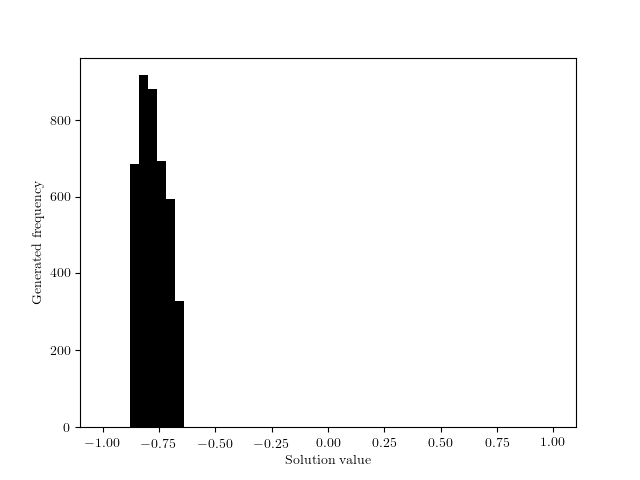
\includegraphics[width=0.6\textwidth]{initialisedGenerator1}
    \end{subfigure}
    \begin{subfigure}[a]{1.\textwidth}
        \centering
        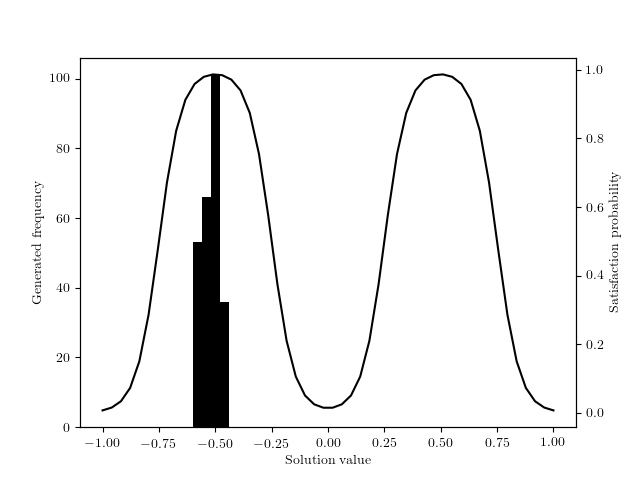
\includegraphics[width=0.6\textwidth]{initialisedGenerator2}
    \end{subfigure}
    \begin{subfigure}[a]{1.\textwidth}
        \centering
        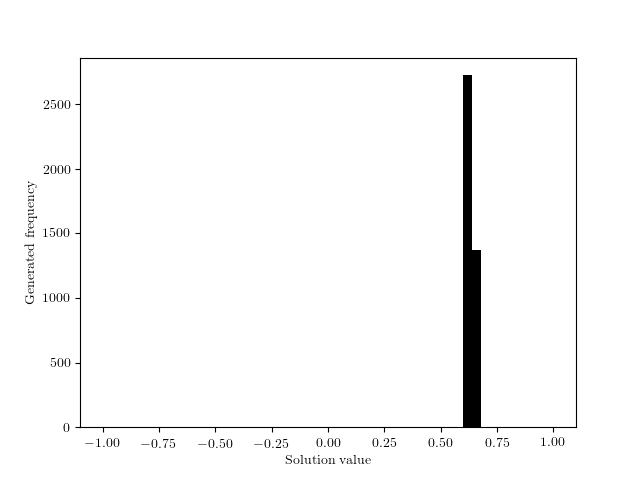
\includegraphics[width=0.6\textwidth]{initialisedGenerator3}
    \end{subfigure}
    \caption{
        $\hat{V'_c}$ immediately after initialisation for three different seeds.
        4096 histogram samples were taken instead of 256.
    }
\label{fig:initialisedGenerator}
\end{figure}
Pretraining is performed in the same way as normal training, but one of the spread losses $q_\text{id}$ or $q_\text{sep}$ is minimised instead of $\hat{p}$.
Because the spread is a subjective quality which cannot be objectively measured, the success of each spread metric will be judged on whether it enables $g'$ to learn both modes of $\hat{V_c}$ simultaneously.

Below are examples of typical $\hat{V'_c}$ after pretraining with each spread metric.
\begin{figure}[H]
    \begin{center}
    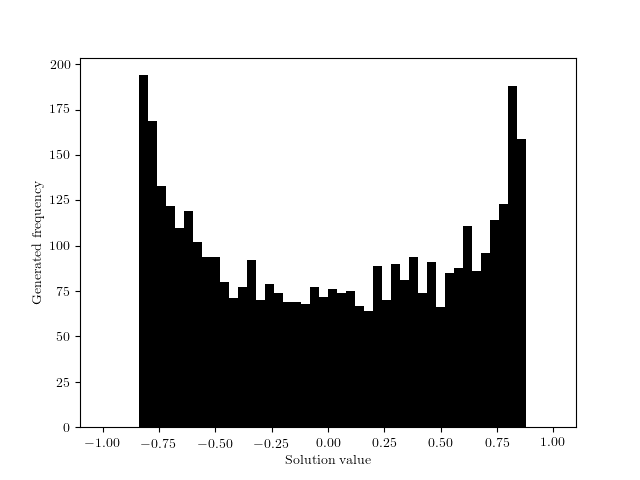
\includegraphics[width=\textwidth]{identitySpread}
    \caption{
        $\hat{V'_c}$ after pretraining until convergence using $q_\text{id}$.
        4096 histogram samples were taken instead of 256.
    }
    \label{fig:identitySpread}
    \end{center}
\end{figure}

\begin{figure}[H]
    \begin{center}
    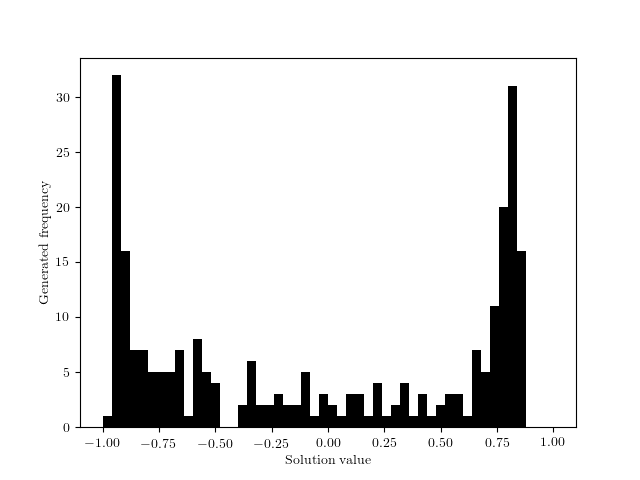
\includegraphics[width=\textwidth]{separationSpread}
    \caption{
        $\hat{V'_c}$ after pretraining until convergence using $q_\text{sep}$.
    }
    \label{fig:separationSpread}
    \end{center}
\end{figure}
Both metrics show signs of causing $g'$ to explore a far greater proportion of $S$ than immediately after initialisation, but also have a tendency to over-explore the boundaries.
This effect is much more pronounced with $q_\text{sep}$.
The true success of each metric, however, is determined by the generator's ability to find different modes when precision is optimised after pretraining.
\begin{figure}[H]
    \begin{center}
    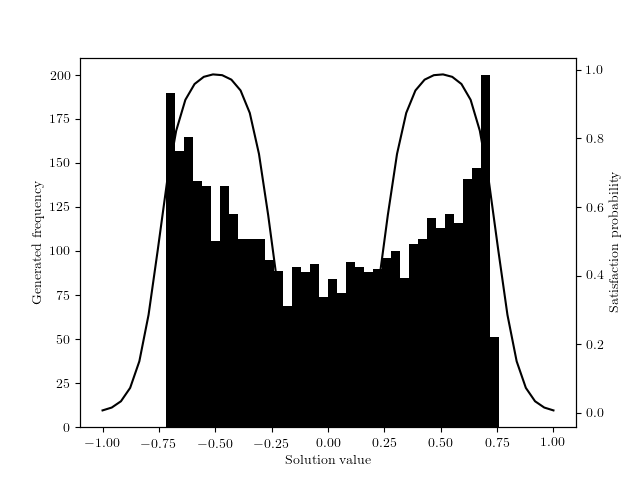
\includegraphics[width=\textwidth]{identityThenPrecision}
    \caption{
        $\hat{V'_c}$ after pretraining until convergence using $q_\text{id}$, then trained to maximise $\hat{p}$ until convergence.
    }
    \label{fig:identityThenPrecision}
    \end{center}
\end{figure}

\begin{figure}[H]
    \begin{center}
    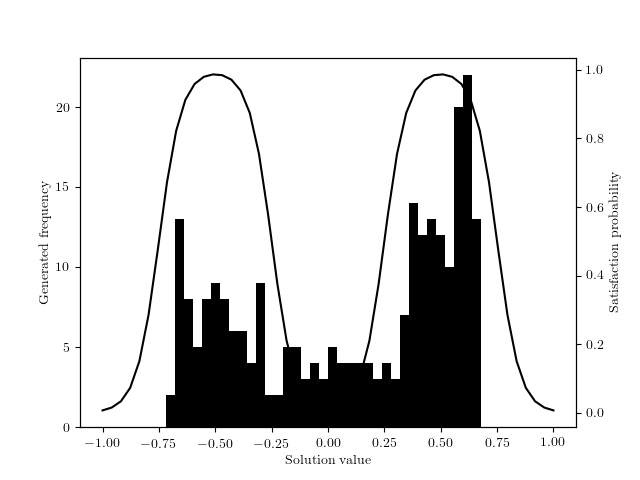
\includegraphics[width=\textwidth]{separationThenPrecision}
    \caption{
        $\hat{V'_c}$ after pretraining until convergence using $q_\text{sep}$, then trained to maximise $\hat{p}$ until convergence.
    }
    \label{fig:separationThenPrecision}
    \end{center}
\end{figure}
Comparing Figure \ref{fig:sigmoidBumpHistogramBimodal} to Figures \ref{fig:identityThenPrecision} and \ref{fig:separationThenPrecision} it is clear that pretraining greatly enhances the generator's ability to sample multiple modes.
This comes at a cost, however; while the generator pretrained on $q_\text{id}$ samples approximately equally from both modes, it also frequently samples solutions from between the modes which are unlikely to satisfy $h$.

\subsection{Maximising precision and spread} \label{subsection:maximisingPrecisionAndSpread}

All experiments in this section used the parameters in Appendix \ref{appendix:precisionOptimisationTrainingParameters}.

Another possibility is, after pretraining, to minimise a weighted sum of $\hat{p}$ and $q$, as if the spread loss were a substitute for $\hat{r}$.
Using $q_\text{id}$, this has an intuitive explanation: $q_\text{id}$ penalises the relocation of probability mass between $L$ and $S$, thereby providing an incentive to $g'$ to seek out areas of high satisfaction probability which are more local.

Figure \ref{fig:identityAndPrecision} shows $\hat{V'_c}$ after $q_\text{id}$ pretraining, then training to minimise $\hat{p}+q_\text{id}$ until convergence.
\begin{figure}[H]
    \begin{center}
    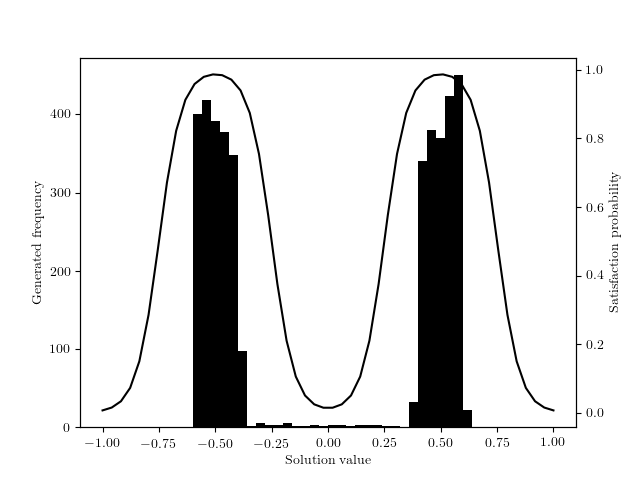
\includegraphics[width=\textwidth]{identityAndPrecision}
    \caption{
        $\hat{V'_c}$ after pretraining, followed by training to maximise $\hat{p}+q_\text{id}$ until convergence.
    }
    \label{fig:identityAndPrecision}
    \end{center}
\end{figure}
This is clearly a result superior to any obtained previously, with $\hat{V'_c}$ covering both modes, and almost always in regions with a satisfaction probability above $0.8$.
Solutions less likely to satisfy $h$ are almost never sampled.

\subsection{Constraint embeddings} \label{subsection:constraintEmbeddings}

The only part of the proposed architecture that has yet to be verified is the insertion of constraints in an embedded form at the output layer of the generator.
This is achieved using a generalised alteration of $h$ introduced in Appendix \ref{appendix:bimodalCSF} such that the position of each peak is controlled by one component of $c$.
Code for replicating this function is reproduced in Appendix \ref{appendix:tensorflowCSF} and training was performed with parameters in Appendix \ref{appendix:embedderVerificationParameters}.

Generally, $\hat{V'_c}$ was able to adapt to account for the differences in $h$.
Not only was it often able to distinguish between two modes, but also adjusted its mapping appropriately when the two peaks were near each other and so merged into one mode.
\begin{figure}[H]
    \centering
    \begin{subfigure}[a]{1.\textwidth}
        \centering
        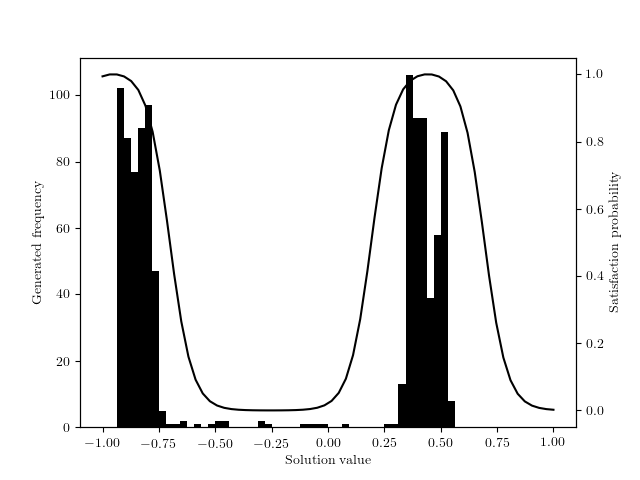
\includegraphics[width=0.6\textwidth]{embeddedConstraint1}
    \end{subfigure}
    \begin{subfigure}[a]{1.\textwidth}
        \centering
        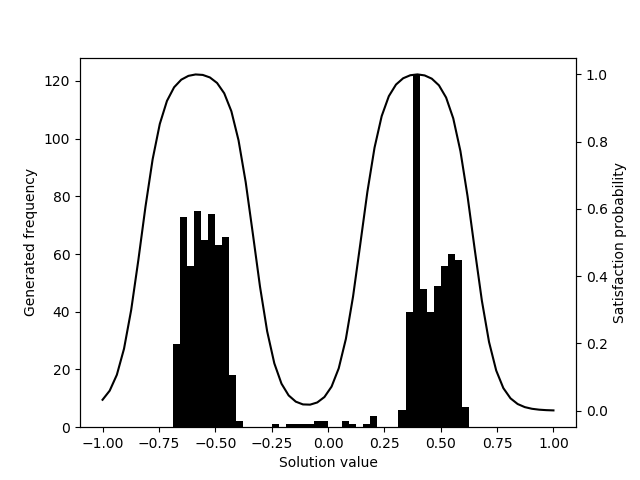
\includegraphics[width=0.6\textwidth]{embeddedConstraint2}
    \end{subfigure}
    \begin{subfigure}[a]{1.\textwidth}
        \centering
        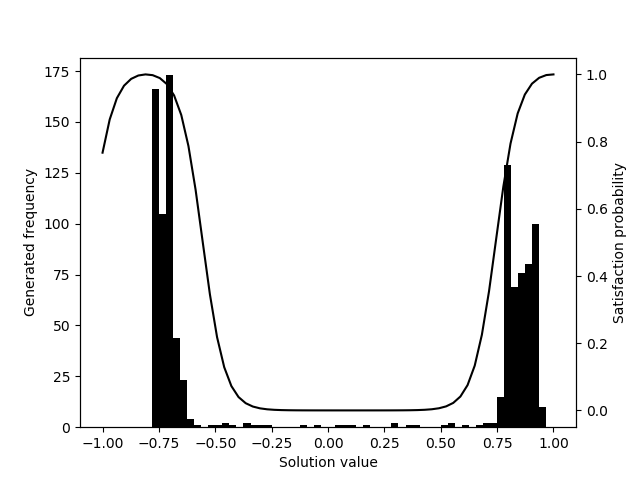
\includegraphics[width=0.6\textwidth]{embeddedConstraint5}
    \end{subfigure}
    \caption{
        Examples of a generator learning to adjust its mapping to changing constraints.
    }
\label{fig:embeddedConstraintsBimodal}
\end{figure}
Occasionally, when large regions of $S$ did not satisfy $c$, poor mapping choices such as those observed in Figure \ref{fig:embeddedConstraintTooSparse} would occur.
It is hypothesised that these are artefacts of the cost of moving probability mass from one side of $S$ to the other became greater than the gain in precision; this is partially confirmed by observations that this error happened less frequently once $w$ was reduced.
\begin{figure}[H]
    \begin{center}
    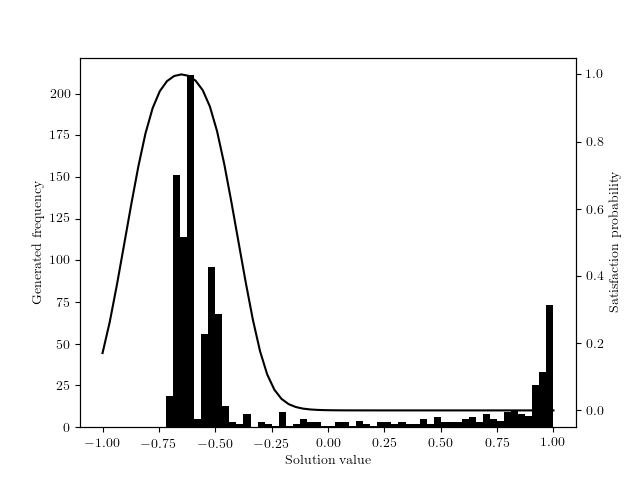
\includegraphics[width=\textwidth]{embeddedConstraint4}
    \caption{
        An example of a constraint whose viable space was so small compared to $S$ that $g'$ was forced to sample poor solutions to prevent penalties from $q_\text{id}$.
        This can be prevented by reducing $w$.
    }
    \label{fig:embeddedConstraintTooSparse}
    \end{center}
\end{figure}
\begin{figure}[H]
    \begin{center}
    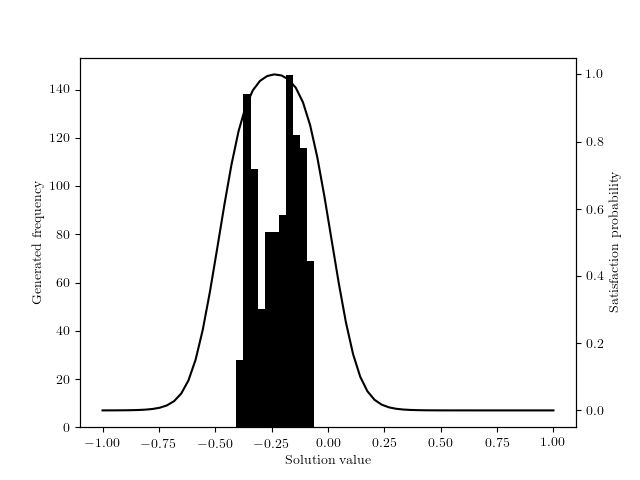
\includegraphics[width=\textwidth]{embeddedConstraint7}
    \caption{
        A constraint for which two peaks join together into a single peak, which is accurately reflected in $\hat{V'_c}$.
    }
    \label{fig:embeddedConstraintJoinedModes}
    \end{center}
\end{figure}

\section{Method properties} \label{section:methodProperties}

The first half of this chapter described experiments performed on abstract, simplified engineering problems to inform the design of the project's deliverable architecture.
The remainder of this chapter will examine that architecture's performance in more depth and in more complex engineering environments.

\subsection{Expected satisfaction probability} \label{subsection:expectedSatisfactionProbability}

One crucial requirement of $\hat{V'_c}$ is that the solutions it produces should satisfy $c$.
The expected satisfaction probability (ESF) will be used to measure the performance of the generator on various environments, and is calculated by taking the mean of $h'(c,s)$ over a batch of sampled solutions.
Similarly, the median satisfaction probability (MSF) is the median $h'(c,s)$ of every solution in the batch.

\subsection{Relative density of true solutions} \label{subsection:relativeDensityOfTrueSolutions}

Another requirement of $\hat{V'_c}$ is that it samples from the entire range of viable solutions.
In all further experiments, either $q_\text{id}$ or $q_\text{sep}$ is used as a subtitute for $\hat{r}$ due to its intractibility.
For the purposes of evaluating the generator's performance, the relative density of true solutions in $\hat{V'_c}$ will be calculated.

Calculating this value requires a sample of solutions from $\hat{V_c}$; this is achieved using the Metropolis-Hastings algorithm \cite{robert16}.
Finding the relative density of each of these solutions in $\hat{V'_c}$ requires creating an $n$-tree (a generalisation of a quadtree to an arbitrary number of dimensions) from a large number of samples from $g'$.
For each true solution sampled from the Markov chain, the smallest bin within the $n$-tree containing that solution is found.
The relative density of that solution is then defined as:
\begin{equation}
    \text{relative density}=\rho=\frac{\text{population of bin}/\text{population of whole tree}}{\text{volume of bin}/\text{volume of }S}
\end{equation}
Intuitively, if a solution has a relative density greater than $1$ then it is being sampled more frequently than it would be if the generator simply output a uniform distribution; conversely, a relative density of less than $1$ suggests it is being sampled less frequently.
For a generator with good recall it could therefore be expected that the mean relative density over a sample of solutions taken from $\hat{V_c}$ by a MCMC algorithm should be above $1$.

\subsection{Data collection} \label{subsection:dataCollection}

All environments used in further experiments implemented a common interface that allowed the training of a generator upon them to output a large JSON file containing data about the experiment parameters and results.
An exemplar JSON file is shown in Appendix \ref{appendix:exampleJSON}, but the results were not reproduced here in full due to their excessive size.

\subsection{Effect of recall weight} \label{subsection:effectOfRecallWeight}

A generator was trained on a more concrete engineering environment to examine the effect of tuning $w$ on the tradeoff between precision and recall.
It is hypothesised that low $w$ causes high satisfaction probability but low relative density, whereas high $w$ causes the opposite.

The holes environment (Appendix \ref{appendix:holesEnvironment}) was used to test this hypothesis.
Datasets of $(c,s,h(c,s))$ tuples were created to train the discriminator, balanced such that roughly half of the examples were positives: samples were taken uniformly from $S$ and $C$, and the satisfaction probability was calculated for each pair.
The training parameters used are reproduced in Appendix \ref{appendix:holesTrainingParameters}.
\begin{figure}[H]
    \begin{center}
    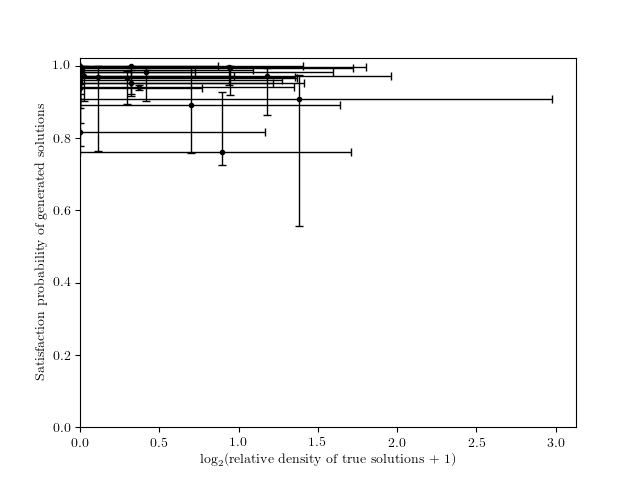
\includegraphics[width=\textwidth]{solutionPropertiesEvenlyWeighted}
    \caption{
        The median and interquartile range of the satisfaction probability and relative density of 128 generated and 128 true solutions to a sample of constraints.
        Relative density is given as $\log_2(\rho+1)$ to space the data while conserving the important lines $\rho=0$ and $\rho=1$.
        Generator trained with $w=1$.
    }
    \label{fig:solutionPropertiesEvenlyWeighted}
    \end{center}
\end{figure}
Immediately noticeable is the very high precision: only one of the constraints has a satisfaction probability of under $0.8$ for at least half of its generated solutions.
Recall is generally quite poor, however.
Only a small proportion of the true solutions were sampled more frequently by $\hat{V'_c}$ than by a uniform distribution.
The hypothesis suggests that increasing $w$ would shift the constraints to regions of higher $\rho$, at the cost of slightly decreasing $\hat{p}$.
\begin{figure}[H]
    \begin{center}
    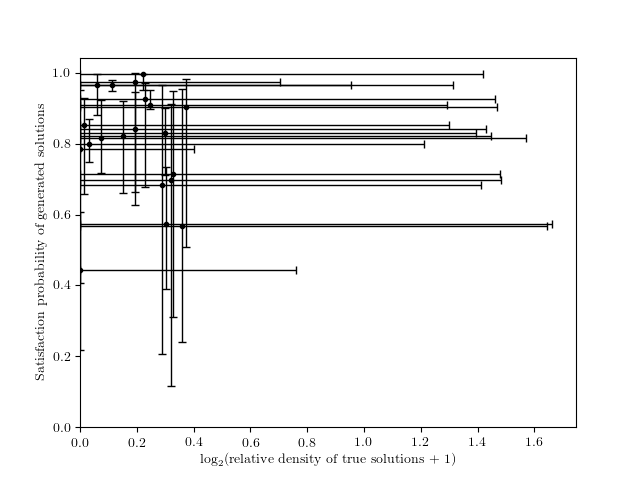
\includegraphics[width=\textwidth]{solutionPropertiesW3}
    \caption{
        The median and interquartile range of the satisfaction probability and relative density of 128 generated and 128 true solutions to a sample of constraints.
        Generator trained with $w=3$.
    }
    \label{fig:solutionPropertiesW3}
    \end{center}
\end{figure}
Figure \ref{fig:solutionPropertiesW3} shows this to be partially incorrect, however: while a reduction in satisfaction probability is observed, increasing $w$ does not appear to have increased the relative density for the majority of constraints.
But the spread loss does appear to be consistently reduced by increasing $w$ (Table \ref{table:generatorTrainingProgression}), suggesting that $q_\text{id}$ is not an accurate gauge of recall.
That increasing $w$ did trade precision for spread does suggest, however, that if a better substitute for recall could be obtained, tuning $w$ might have the intuitive effect hypothesised previously.
\begin{table}[H]
    \centering
    \begin{tabular}{*6c}
    \toprule
    {} & {} & \multicolumn{2}{c}{After pretraining} & \multicolumn{2}{c}{After training}\\
    Experiment&$w$&Spread loss&Precision loss&Spread loss&Precision loss\\
    \midrule
    1&0.500&0.116&-0.452&0.213&-0.650\\2&0.500&0.092&-0.503&0.156&-0.643\\3&0.500&0.098&-0.466&0.225&-0.647\\4&0.500&0.103&-0.391&0.300&-0.638\\5&0.500&0.119&-0.410&0.229&-0.637\\6&1.000&0.103&-0.420&0.173&-0.632\\7&1.000&0.093&-0.324&0.181&-0.659\\8&1.000&0.091&-0.537&0.174&-0.644\\9&1.000&0.136&-0.457&0.136&-0.631\\10&1.000&0.113&-0.438&0.143&-0.634\\11&2.000&0.121&-0.452&0.113&-0.549\\12&2.000&0.104&-0.431&0.132&-0.600\\13&2.000&0.085&-0.435&0.105&-0.515\\14&2.000&0.090&-0.435&0.164&-0.617\\15&2.000&0.110&-0.429&0.124&-0.591\\16&3.000&0.074&-0.442&0.100&-0.558\\
    17&3.000&0.088&-0.443&0.121&-0.544\\18&3.000&0.123&-0.444&0.108&-0.551\\19&3.000&0.100&-0.423&0.099&-0.511\\20&3.000&0.103&-0.427&0.111&-0.487\\
    \bottomrule
    \end{tabular}
    \caption{$\hat{p}$ and $q_\text{id}$ at different points throughout training.}
    \label{table:generatorTrainingProgression}
\end{table}

\subsection{Equality constraints} \label{subsection:equalityConstraints}

A common constraint in engineering problems is an equality constraint, specifying a property of a design must equal a particular value.
Such a constraint can be created using the proposed architecture by parameterising the constraint such that it limits the upper and lower acceptable bounds of a property, and then setting these two bounds to be arbitrarily close together.

The Branin function, $\beta(x,y)$, was chosen to test the ability of the generator to approximate equality constraints as it is a standard test function for which an equality constraint produces distinct contours (Appendix \ref{appendix:braninFunction}).
Having a solution dimension of $2$ also makes visualisation of the results possible.
To make passing the function and its arguments into the discriminator possible, both inputs and the output were scaled to be in $[0,\;1]$.
The constraint vector, in two dimensions, was then defined such that the constraint is considered satisfied when:
\begin{equation}
    c_1\cdot c_2\le\beta(x,y)\le c_2,\quad c_1,c_2\;\in\;[0,\;1]
\end{equation}
and so:
\begin{equation}
    h(c,s)=\left\{\begin{array}{ll}\text{satisfied}&\mbox{if }c_1\cdot c_2\le\beta(s_1,s_2)\le c_2\\\text{unsatisfied}&\mbox{otherwise}\end{array}\right.
\end{equation}
As with the environment in \S\ref{subsection:effectOfRecallWeight}, datasets of various sizes were created and the proposed architecture was trained on the resulting data.
Training parameters can be found in Appendix \ref{appendix:braninTrainingParameters}.
The generator produced good solutions over a large range of $V_c$ for most constraints, but was unable to find solutions to some constraints, as shown in Figure \ref{fig:braninPropertiesW3}.
\begin{figure}[H]
    \begin{center}
    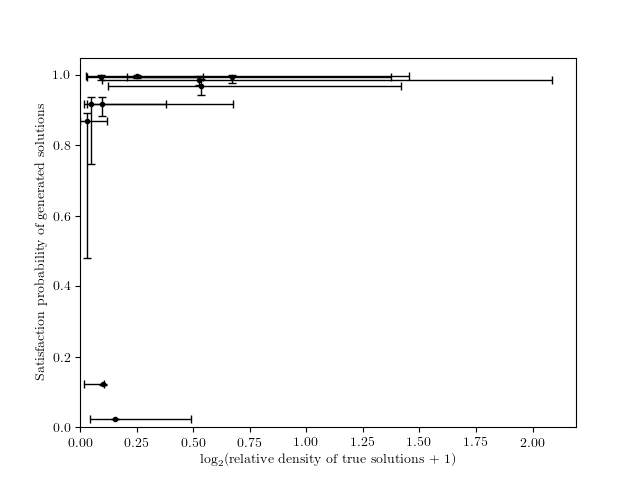
\includegraphics[width=\textwidth]{braninPropertiesW1}
    \caption{
        Solutions to a bounded Branin function, as sampled from $5$ different instances of $\hat{V'_c}$.
    }
    \label{fig:braninPropertiesW3}
    \end{center}
\end{figure}
After training, the constraint $c=[0.5,\;0.5]$ was chosen, corresponding to regions of the solution space for which $\beta'$ outputs values in $[0.25,\;0.5]$.
Samples were then drawn from $\hat{V'_c}$ and plotted in $S$, with overlays for the output of both $h'$ and $h$, in Figure \ref{fig:equality05}.
\begin{figure}[H]
    \begin{center}
    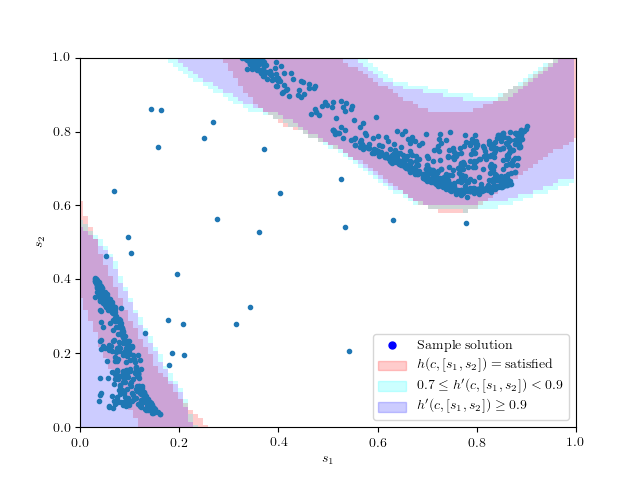
\includegraphics[width=\textwidth]{equality05}
    \caption{
        1024 sample solutions, high-likelihood regions of the discriminator, and the regions containing true solutions for a generator trained on the bounded Branin function environment.
        $c=[0.5\;0.5]$.
    }
    \label{fig:equality05}
    \end{center}
\end{figure}
It is immediately clear that the vast majority of sampled solutions lie within regions of $S$ which the discriminator predicts are likely to satisfy $c$.
Note also that $h'$ appears to have regions of very steep gradients (the cyan region in Figure \ref{fig:equality05} is thin compared to the blue region) and is generally accurate in its prediction of the boundaries of $V_c$.
While the points are spread out sufficiently to cover much of $V_c$ and avoid coalescing into peaks, there are also regions near the periphery of $V_c$ which are undersampled, suggesting that some precision could be traded for an increase in recall.

Increasing $c_1$ to $0.7$, constraining $V_c$ to those solutions for which $0.35\le\beta'(s)\le0.5$, yields similar results (Figure \ref{fig:equality07}).
\begin{figure}[H]
    \begin{center}
    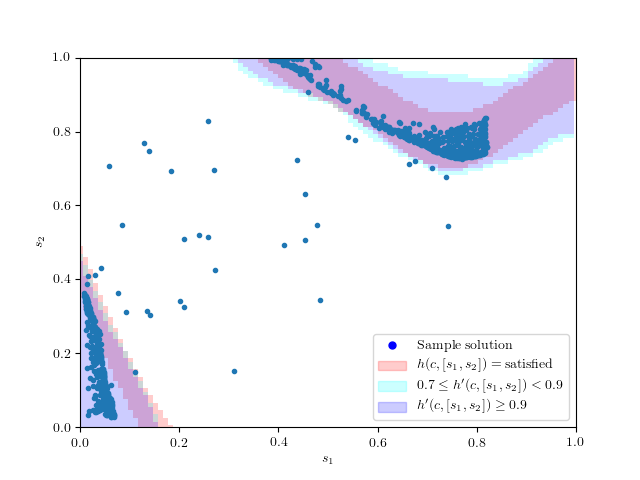
\includegraphics[width=\textwidth]{equality07}
    \caption{
        1024 sample solutions, high-likelihood regions of the discriminator, and the regions containing true solutions for a generator trained on the bounded Branin function environment.
        $c=[0.7,\;0.5]$.
    }
    \label{fig:equality07}
    \end{center}
\end{figure}
The discriminator's predictions appear to be becoming less accurate as the bounded constraint approaches an equality constraint, failing to recognise that solutions near the origin do not satisfy $c$.
While the discriminator made similar misclassifications for $c=[0.5,\;0.5]$, the error is now affecting $\hat{V'_c}$ to the extent that a large number of samples are drawn from a region outside $V_c$.

Finally, $c_1$ was increased to $0.9$, representing regions for which $0.45\le\beta'(s)\le0.5$, effectively mimicking an equality constraint (Figure \ref{fig:equality09}).
Of the two modes of $V_c$, one is fairly consistently sampled by $\hat{V'_c}$, while the other is missed almost entirely.
It should be noted that the generator has learned to sample high-likelihood regions of $h'$, but that the discriminator misclassified the mode closer to the origin.
This presents promising evidence that, with further refinement of $h'$, the proposed architecture could be used to accurately sample equality constraints.
\begin{figure}[H]
    \begin{center}
    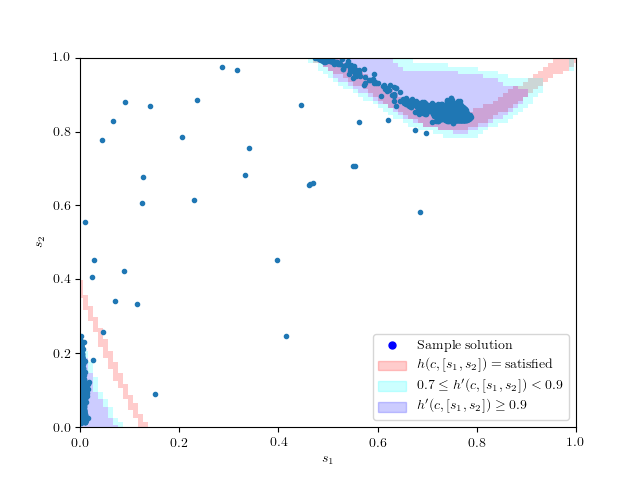
\includegraphics[width=\textwidth]{equality09}
    \caption{
        1024 sample solutions, high-likelihood regions of the discriminator, and the regions containing true solutions for a generator trained on the bounded Branin function environment.
        $c=[0.9,\;0.5]$.
    }
    \label{fig:equality09}
    \end{center}
\end{figure}

\section{Latent space visualisation} \label{section:latentSpaceVisualisation}

To gain an intuitive understanding of how $g'$ maps $L\mapsto S$, a tool was written to plot invariants of each dimension of $L$ in $S$.
$V_c$ was overlayed onto these plots.
Because both its solution and constraint spaces are two-dimensional, the bounded Branin function environment was considered the most apt for visualisation purposes, and so the generator trained in that environment was used.
\begin{figure}[H]
    \begin{center}
    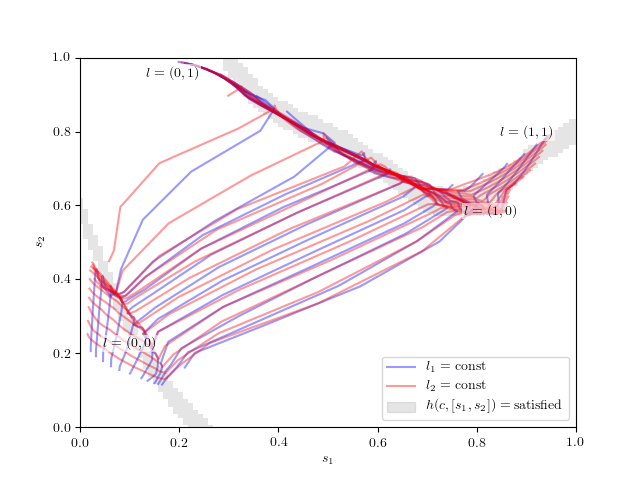
\includegraphics[width=\textwidth]{latentPlot0803}
    \caption{
        Latent invariants in the solution space of the bounded Branin environment for $c=[0.8,\;0.3]$.
    }
    \label{fig:latentPlot0803}
    \end{center}
\end{figure}
Figure \ref{fig:latentPlot0803} shows a highly constrained case where two distinct, narrow bands of viable solutions exist.
As expected given previous results, the latent space is highly compressed within these two regions, with a sparse region between them.
\begin{figure}[H]
    \begin{center}
    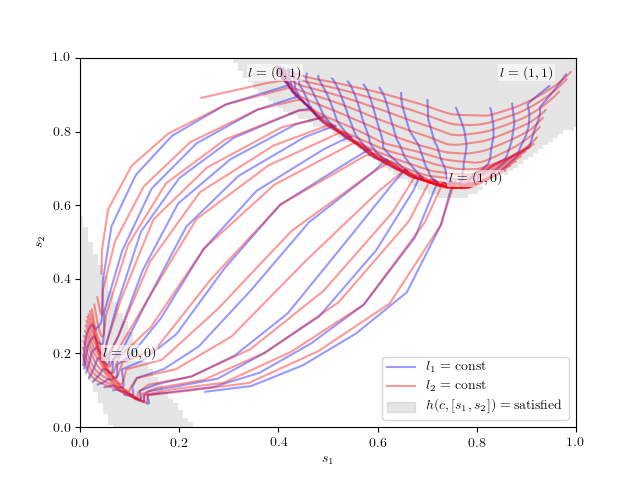
\includegraphics[width=\textwidth]{latentPlot0407}
    \caption{
        Latent invariants in the solution space of the bounded Branin environment for $c=[0.4,\;0.7]$.
    }
    \label{fig:latentPlot0407}
    \end{center}
\end{figure}
The near-equality constraint is relaxed somewhat in Figure \ref{fig:latentPlot0407}, giving way to much larger areas of viable solutions.
The latent space is, correctly, more spread out in this plot, but some parts of $S$ $-$ including some viable solutions $-$ exist completely outside $L$.
This might explain why, in \S\ref{subsection:effectOfRecallWeight}, so many true solutions were found to have no likelihood of occurring in $\hat{V'_c}$.
\begin{figure}[H]
    \begin{center}
    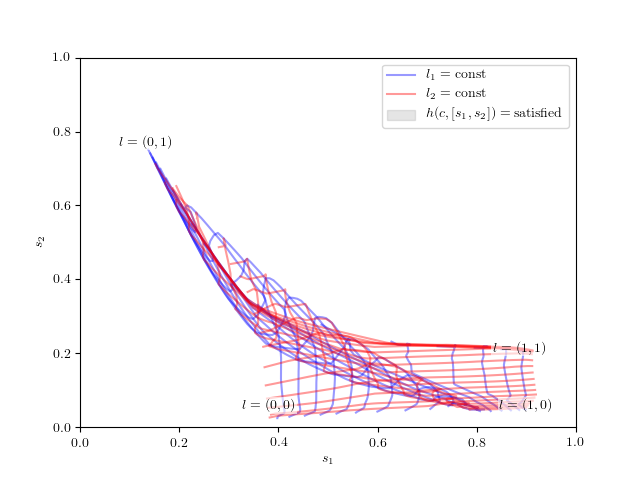
\includegraphics[width=\textwidth]{latentPlot0000}
    \caption{
        Latent invariants in the solution space of the bounded Branin environment for $c=[0.0,\;0.0]$, a degenerate case with no solutions.
    }
    \label{fig:latentPlot0000}
    \end{center}
\end{figure}
For the sake of completeness, Figure \ref{fig:latentPlot0000} shows the behaviour of $g'$ in a degenerate case with no solutions.
Far fewer sparse regions appear here than in the other examples, with the entirety of $L$ relatively compressed.
It also appears to frequently overlap itself, a phenomena not frequently seen for other constraints.
\begin{figure}[H]
    \begin{center}
    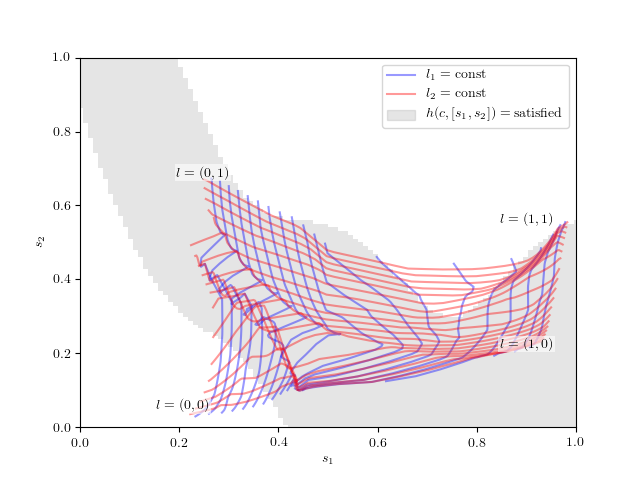
\includegraphics[width=\textwidth]{latentPlot0001}
    \caption{
        Latent invariants in the solution space of the bounded Branin environment for $c=[0.0,\;0.1]$.
    }
    \label{fig:latentPlot0001}
    \end{center}
\end{figure}
Finally, Figure \ref{fig:latentPlot0001} shows a fairly lenient case with a ride range of potential solutions.
Here, poor recall is particularly evident, with relatively few of the potential solutions having latent equivalents in spite of the fact that most of $L$ maps to a viable solution.

\end{document}
